\documentclass[12pt,a4paper]{article}
\usepackage[utf8]{inputenc}
\usepackage[utf8]{vietnam} %Bien dich duoc tieng Viet
\usepackage{amsmath,amsfonts,amssymb} %Font toan
\usepackage{type1cm}
\usepackage{subfig}
\usepackage{graphicx}
\graphicspath{ {images/} }
\usepackage{enumerate}
\usepackage[unicode]{hyperref} %Tu dong tao bookmark
\usepackage{indentfirst} %Thut vao dau dong o tat ca cac doan
\usepackage{comment}
\usepackage{listings} %Dinh dang code
\usepackage{color} %Mau sac
\usepackage[left=2cm,right=2cm,top=2cm,bottom=2cm]{geometry} %Canh lề trái - phải - trên - dưới cho tài liệu
\usepackage{multirow}
\usepackage{hyperref}
\hypersetup{
%    colorlinks=true,
%    linkcolor=blue,
    filecolor=magenta,      
    urlcolor=cyan,
}
\renewcommand{\arraystretch}{1.3}
\definecolor{dkgreen}{rgb}{0,0.6,0}
\definecolor{gray}{rgb}{0.5,0.5,0.5}
\definecolor{mauve}{rgb}{0.58,0,0.82}

\lstset{frame=tb,
  language=bash,
  aboveskip=3mm,
  belowskip=3mm,
  showstringspaces=false,
  columns=flexible,
  basicstyle={\small\ttfamily},
  numbers=left,
  numberstyle=\tiny\color{gray},
  keywordstyle=\color{blue},
  commentstyle=\color{dkgreen},
  stringstyle=\color{mauve},
  breaklines=true,
  captionpos=t,
  breakatwhitespace=true,
  tabsize=2
}
\title{\textbf{Raspberry Pi Kiosk Screen}}
\author{GVHD: Huỳnh Nguyễn Xuân Cần \qquad SVTH: Thi Minh Nhựt}
\date{Thời gian: Ngày 16 tháng 07 năm 2016}

\begin{document}
\pagenumbering{gobble}
\maketitle
\tableofcontents
\newpage
\pagenumbering{arabic}
\setcounter{page}{1}
\section{Các thiết lập cần thiết}
\subsection{Enable SSH}
	Khi muốn điều khiển Raspberry Pi không cần kết nối chuột, bàn phím và màn hình, chọn điều khiển qua \verb|SSH| (điều kiện có kết nối Internet):

	\begin{list}{--}{}
		\item Mở \verb|raspi-config|:
			\begin{lstlisting}[language=bash]
$ sudo raspi-config
			\end{lstlisting}
		
		\item Chọn \verb|Advanced Options|:
			\begin{figure}[!h]
				\begin{center}
					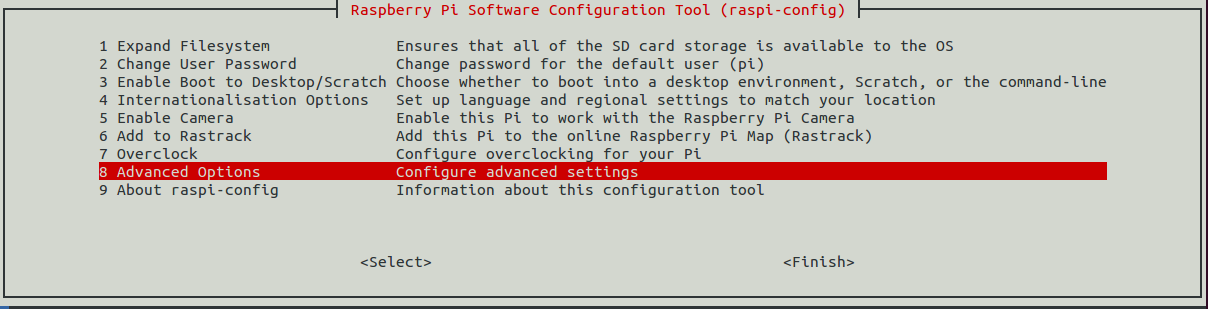
\includegraphics[scale=.3]{Advanced-Options.png}
				\end{center}
				\caption{Advanced Options}
			\end{figure}

		\item Chọn \verb|SSH|:
			\begin{figure}[!h]
				\begin{center}
					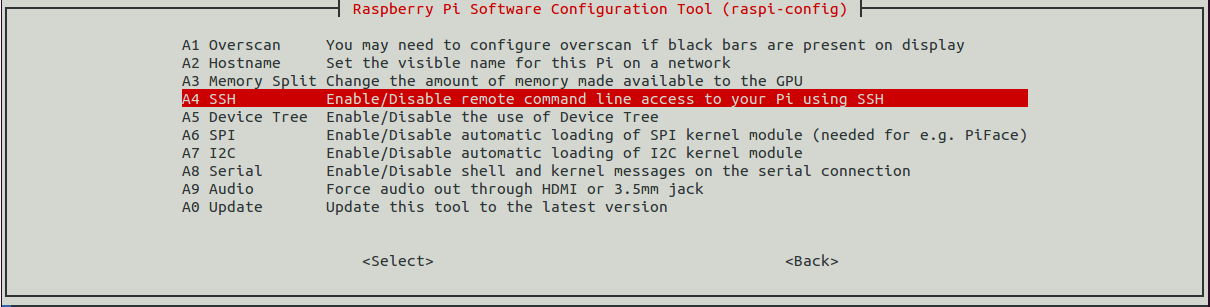
\includegraphics[scale=.3]{SSH.png}
				\end{center}
				\caption{SSH}
			\end{figure}

		\item Chọn \verb|Enable|:
			\begin{figure}[!h]
				\begin{center}
					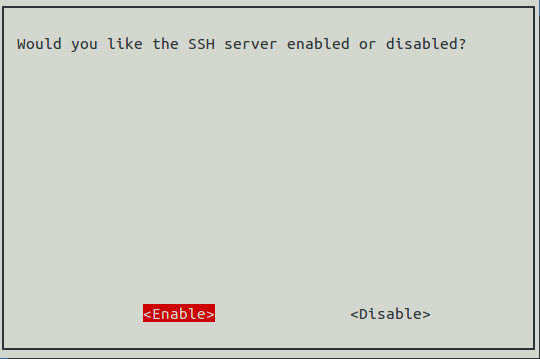
\includegraphics[scale=.3]{Enable-SSH.png}
				\end{center}
				\caption{Enable SSH}
			\end{figure}
	\end{list}
	
\subsection{Expand Filesystem}
	Khi cài đặt hệ điều hành \verb|Raspbian| bằng:
	
	\begin{itemize}
		\item \verb|NOOBS|: thì hệ thống tập tin đã được mở rộng tự động, dung lượng thẻ nhớ được sử dụng tối đa.
		
		\item \verb|SD Cards|: thì dung lượng của thẻ nhớ chỉ sử dụng được hơn $3GB$.
	\end{itemize}

	Để sử dụng dung lượng tối đa của thẻ nhớ, chọn \verb|Expand Filesystem| (để tránh báo lỗi khi cài đặt chương trình do không đủ bộ nhớ).

	\begin{list}{--}{}
		\item[] Mở \verb|raspi-config|:
			\begin{lstlisting}[language=bash]
$ sudo raspi-config
			\end{lstlisting}

			\begin{figure}[!h]
				\begin{center}
					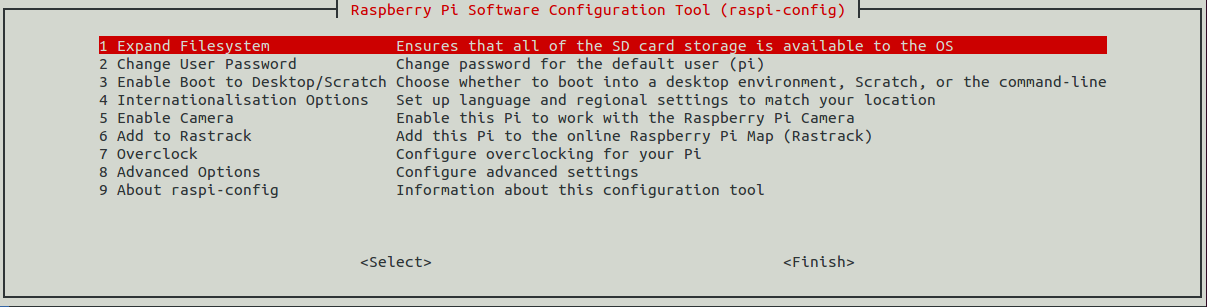
\includegraphics[scale=.3]{Expand-Filesystem.png}
				\end{center}
				\caption{Expand Filesystem}
			\end{figure}
	\end{list}
	
\subsection{Cài đặt kiểu bàn phím}
	Theo mặc định, kiểu bố trí bàn phím của Raspberry Pi theo kiểu Anh, cần thay đổi kiểu bố trí bàn phím theo kiểu Mỹ cho phù hợp.
	
	\begin{list}{--}{}
		\item Mở file \verb|keyboard|
		\begin{lstlisting}[language=bash]
$ sudo nano /etc/default/keyboard
		\end{lstlisting}

		\item Thay đổi nội dung của file như sau:
			\begin{list}{+}{}
				\item Đổi \verb|pc105| thành \verb|pc104|.
				
				\item Đổi \verb|gb| thành \verb|us|.
			\end{list}
		
		\item[$\ast$] Nội dung của file \verb|keyboard| sau khi thay đổi:
			\begin{lstlisting}[language=bash]
# KEYBOARD CONFIGURATION FILE
# Consult the keyboard(5) manual page.
 
XKBMODEL="pc104"
XKBLAYOUT="us"
XKBVARIANT=""
XKBOPTIONS=""
 
BACKSPACE="guess"
			\end{lstlisting}
	\end{list}

\subsection{Change User Password}
	Khi cài đặt hệ điều hành \verb|Raspbian|, thiết lập mặc định: \verb|username: pi| và \verb|password: raspberry|.

	Thay đổi \verb|password| chọn \verb|Change User Password|.
	\begin{list}{--}{}
		\item Mở \verb|raspi-config|:
			\begin{lstlisting}[language=bash]
$ sudo raspi-config
			\end{lstlisting}
			
		\item Chọn \verb|Change User Password|: hình \ref{Fig:Change-user-pass}.
			\begin{figure}[!h]
				\begin{center}
					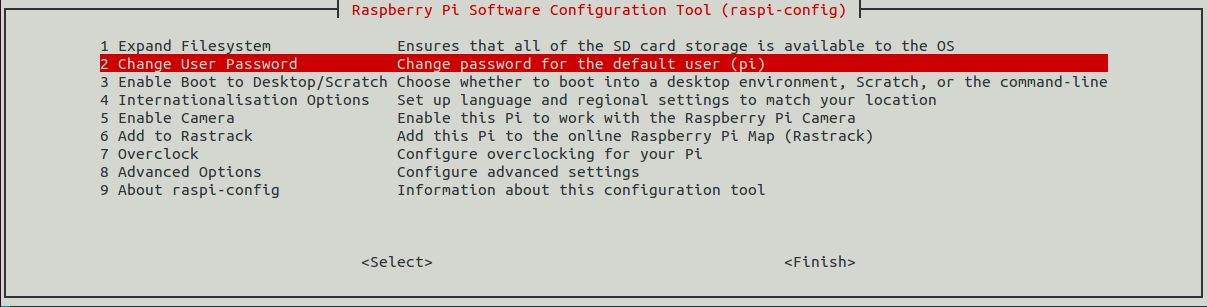
\includegraphics[scale=.3]{Change-user-pass.png} 
				\end{center}
				\caption{Change User Password}\label{Fig:Change-user-pass}
			\end{figure}
			
		\item Nhập \verb|password| mới 2 lần để thay đổi \verb|password| mới (khi nhập ký tự sẽ bị ẩn):
			\begin{lstlisting}[language=bash]
Enter new UNIX password:
Retype new UNIX password:
			\end{lstlisting}
						
		\item Thay đổi thành công sẽ có thông báo:
			\begin{lstlisting}[language=bash]
passwd: password updated successfully
			\end{lstlisting}
	\end{list}
	
\subsection{Internationalisation Options}
	Thay đổi ngôn ngữ, vị trí và múi giờ chọn \verb|Internationalisation Options|.
	\begin{list}{--}{}
		\item Mở \verb|raspi-config|:
			\begin{lstlisting}[language=bash]
$ sudo raspi-config
			\end{lstlisting}
		
		\item Chọn \verb|Internationalisation Options|: hình \ref{Fig:Internationalisation-Options}.
			\begin{figure}[!h]
				\begin{center}
					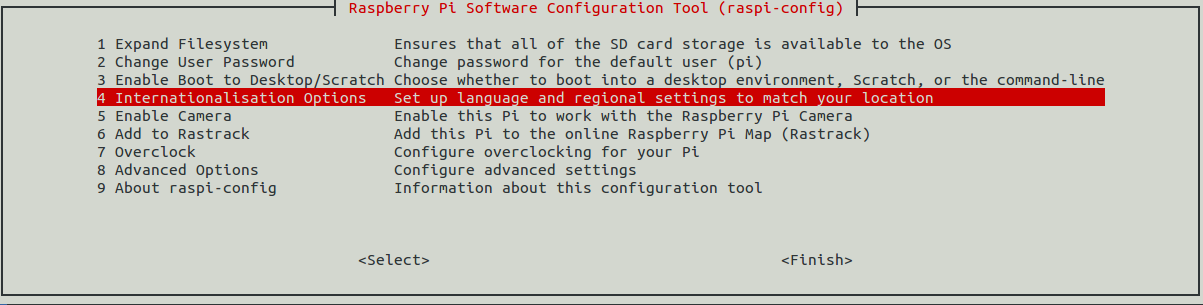
\includegraphics[scale=.3]{Internationalisation-Options.png} 
				\end{center}
				\caption{Internationalisation Options}\label{Fig:Internationalisation-Options}
				\end{figure}
				
		\item Thay đổi ngôn ngữ, chọn \verb|Change Locate|: hình \ref{Fig:Change-locate}. 
		\begin	{list}{+}{}
				\item[$\ast$] Sử dụng phím \verb|space| để chọn hoặc bỏ chọn.
				
				\item Bỏ chọn \verb|en_GB.UTF-8 UTF-8|
				
				\item Chọn \verb|en_US.UTF-8 UTF-8|, như hình \ref{Fig:lang}.
		\end{list}
		
		\begin{figure}[!h]
			\begin{center}
				\subfloat[Chọn Change Locate\label{Fig:Change-locate}]
				{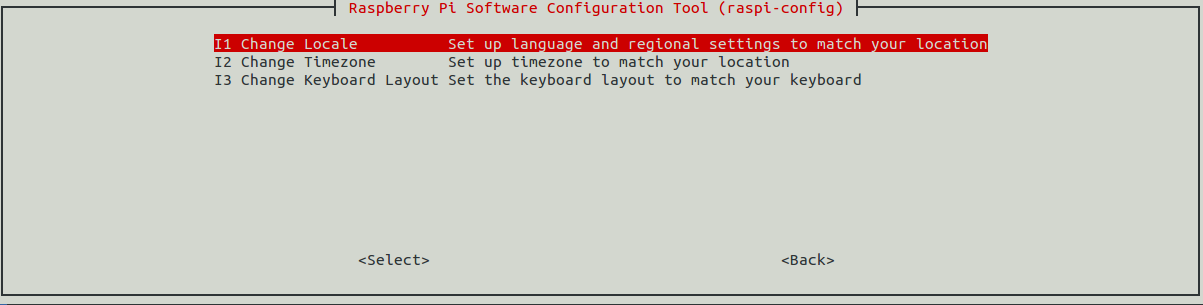
\includegraphics[scale=.27]{Change-locate.png}}\\
				\subfloat[Chọn en\_US.UTF-8 UTF-8\label{Fig:lang}]
				{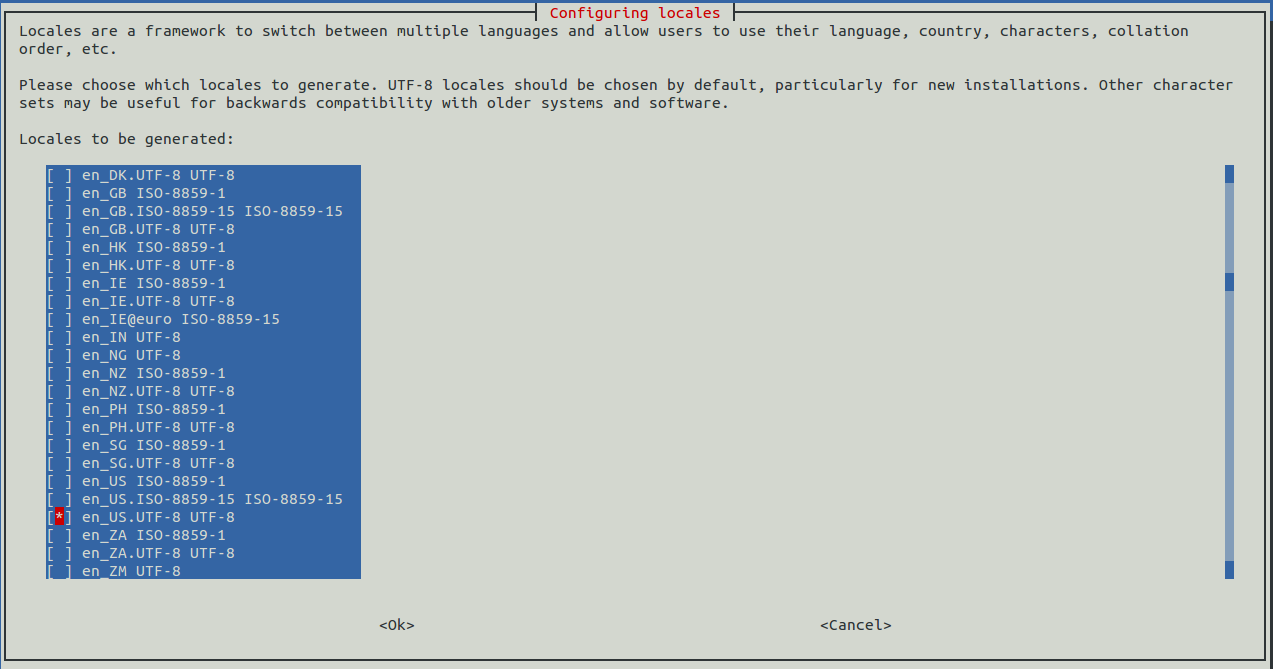
\includegraphics[scale=.25]{lang.png}}	
			\end{center}
			\caption{Change Locate}
		\end{figure}
		
		\item Thay đổi múi giờ, chọn \verb|Change Timezone|: như hình \ref{Fig:Change-Timezone}:
			\begin{list}{+}{}
				\item Chọn \verb|Asia|: hình \ref{Fig:Asia}.
				
				\item Chọn \verb|Ho_Chi_Minh|: hình \ref{Fig:HCM}.
			\end{list}
			
			\begin{figure}[!h]
				\begin{center}
					\subfloat[Chọn Change Timezone\label{Fig:Change-Timezone}]
					{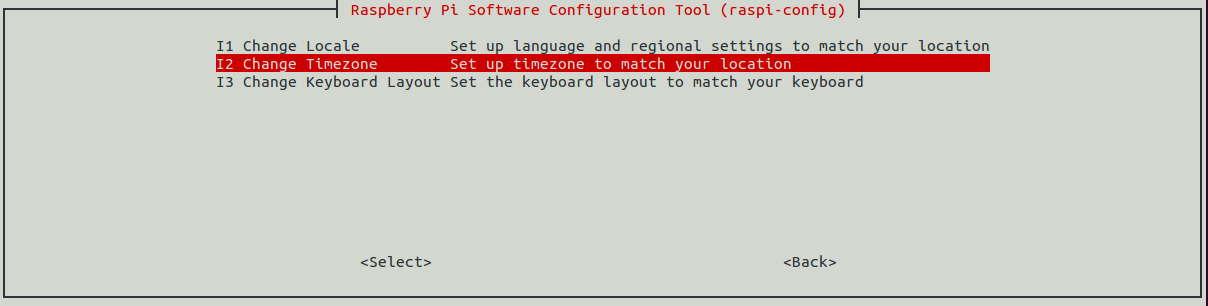
\includegraphics[scale=.3]{Change-Timezone.png}}\\
					\subfloat[Chọn Asia\label{Fig:Asia}]
					{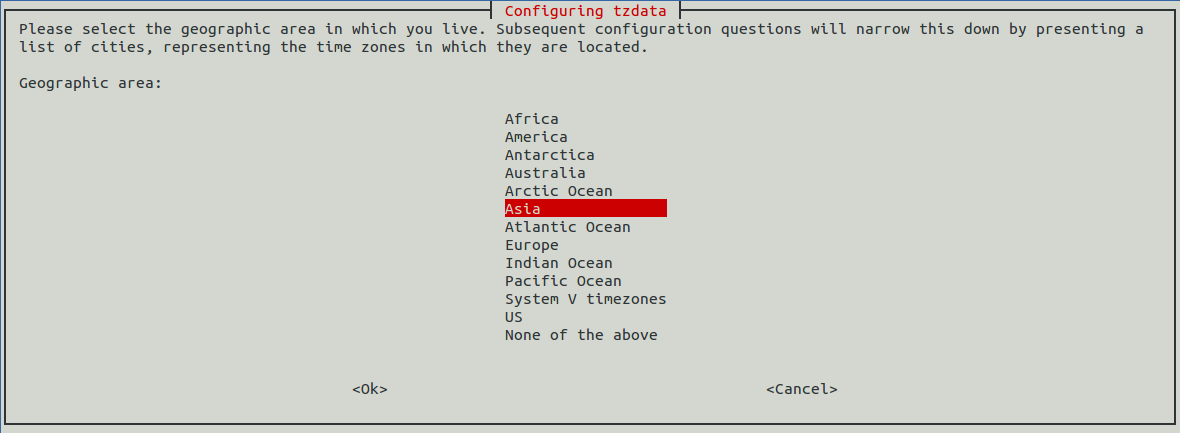
\includegraphics[scale=.3]{Asia.png}}\\
					\subfloat[Chọn Ho\_Chi\_Minh\label{Fig:HCM}]
					{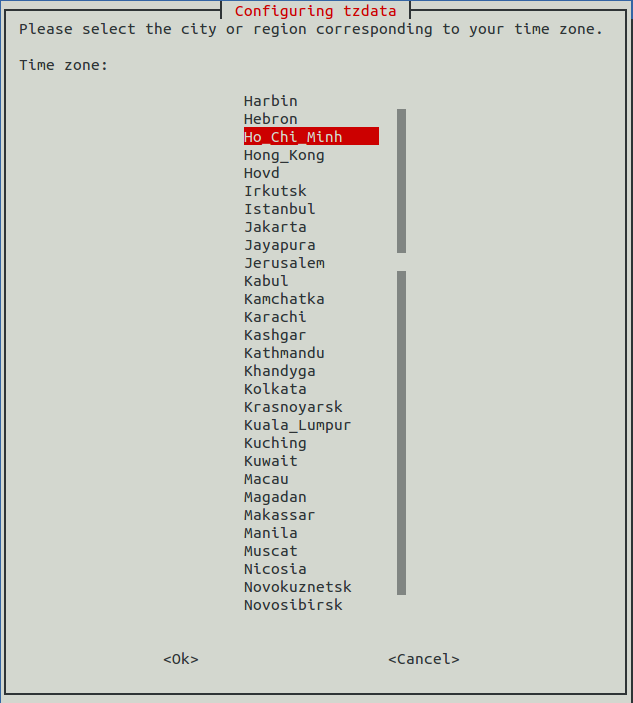
\includegraphics[scale=.3]{HCM.png}}	
				\end{center}
				\caption{Change Timezone}
			\end{figure}
	\end{list}
	
\newpage

\subsection{Tự động đăng nhập khi khởi động}
	Khi khởi động Raspberry Pi sẽ yêu cầu người dùng nhập \verb|username| và \verb|password| để đăng nhập. Để quá trình này tự động, thực hiện như sau:
	\begin{list}{--}{}
		\item Chỉnh sửa nội dung của file \verb|inittab|:
			\begin{list}{+}{}
				\item Mở file \verb|inittab|:
				\begin{lstlisting}[language=bash]
$ sudo nano /etc/inittab
				\end{lstlisting}

				\item Tìm đến dòng \verb|1:2345:respawn:/sbin/getty...| (có thông tin này là được) và thêm dấu \verb|#| vào phía trước, như bên dưới:
					\begin{lstlisting}[language=bash]
#1:2345:respawn:/sbin/getty 115200 tty1
					\end{lstlisting}
				
				\item Thay thế dòng trên bằng dòng sau (vào phía dưới dòng vừa chú thích):
					\begin{lstlisting}[language=bash]
1:2345:respawn:/bin/login -f pi tty1 </dev/tty1 >/dev/tty1 2>&1
					\end{lstlisting}
				
				\item Nhấn \verb|Ctrl + X + Y| để lưu lại thay đổi và thoát.
			\end{list} 
	\end{list}
	
\subsection{Enable Boot to Desktop/Scratch}
	Mặc định Raspberry Pi sau khi khởi động sẽ boot vào giao diện dòng lệnh \verb|Console Text console|.

	Để boot vào giao diện đồ họa chọn \verb|Enable Boot to Desktop/Scratch|
	\begin{list}{--}{}
		\item Mở \verb|raspi-config|:
		\begin{lstlisting}[language=bash]
$ sudo raspi-config
		\end{lstlisting}

		\item Chọn \verb|Enable Boot to Desktop/Scratch|:
			\begin{figure}[!h]
				\begin{center}
					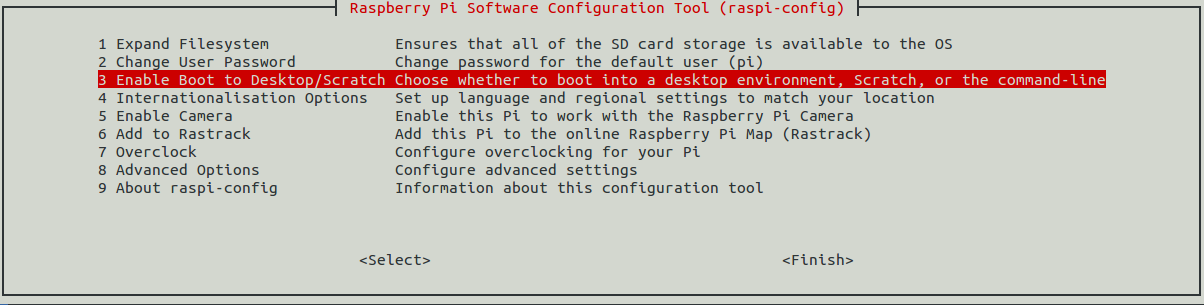
\includegraphics[scale=.35]{Enable-Boot-to-Desktop-Scratch.png}
				\end{center}
				\caption{Enable Boot to Desktop/Scratch}
			\end{figure}
			
		\item Chọn \verb|Desktop Log in as user 'pi' at the graphical desktop| để boot thẳng vào desktop.
		\begin{figure}[!h]
			\begin{center}
				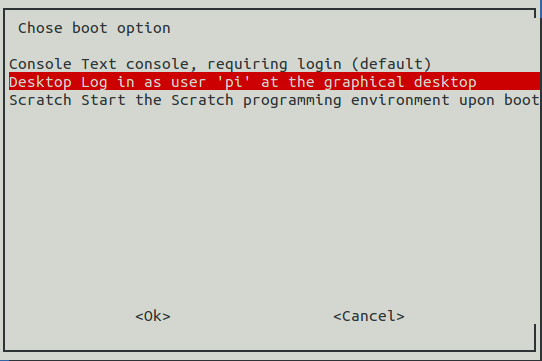
\includegraphics[scale=.35]{desktop.png} 
			\end{center}
			\caption{Desktop Log in as user 'pi' at the graphical desktop}
		\end{figure}
	\end{list}
	
\subsection{Thiết lập cho màn hình hiển thị}
	Tùy vào loại màn hình mà thay đổi các tùy chọn thích hợp trong file \verb|/boot/config.txt|

\section{Xây dựng Raspberry Pi Kiosk Screen}
\subsection{Các hướng dẫn thực hiện}
	\begin{itemize}
		\item Hướng dẫn của \href{http://alexba.in}{Alexba}:

			\begin{footnotesize}
				\url{http://alexba.in/blog/2013/01/07/use-your-raspberrypi-to-power-a-company-dashboard/}
			\end{footnotesize}		
		\item Hướng dẫn của \href{https://www.danpurdy.co.uk}{Danpurdy}:

			\begin{footnotesize}
				\url{https://www.danpurdy.co.uk/web-development/raspberry-pi-kiosk-screen-tutorial/}
			\end{footnotesize}
		
		\item Hướng dẫn của \href{https://github.com/elalemanyo}{Elalemanyo}:

			\begin{footnotesize}
				\url{https://github.com/elalemanyo/raspberry-pi-kiosk-screen}
			\end{footnotesize}
		
		\item Hướng dẫn của \href{http://pi.bek.no}{pi.bek.no}:

			\begin{footnotesize}
				\url{http://pi.bek.no/hideBootMessages/}
			\end{footnotesize}
	\end{itemize}
	
\subsection{Nội dung và kết quả}
\subparagraph{Nội dung}
	\begin{list}{--}{}
		\item Khởi động trực tiếp vào giao diện đồ họa.
		
		\item Khởi động \verb|Chromium| ở chế độ \verb|Kiosk| và vào trực tiếp Web ở chế độ Full Screen.
		
		\item Vô hiệu hóa chế độ \verb|sleep| của màn hình.
		
		\item Ẩn đi con trỏ chuột.
		
		\item Ẩn logo và text khi Raspberry Pi khởi động.
		
		\item Ẩn Task Bar.
	\end{list}

\subparagraph{Hạn chế}Còn khởi động vào Desktop của Raspberry Pi rồi mới khởi động vào địa chỉ Web.

\subsection{Xây dựng Raspberry Pi Kiosk Screen trên Chromium Browser}
	\begin{itemize}
		\item Cài đặt \verb|x11-server-utilities|:
			\begin{lstlisting}[language=bash]
$ sudo apt-get install x11-server-utilities
			\end{lstlisting}

		\item Cài đặt \verb|Chromium|:
			\begin{lstlisting}[language=bash]
$ sudo apt-get install chromium ttf-mscorefonts-installer
			\end{lstlisting}			
			Gói lệnh \verb|ttf-mscorefonts-installer|: cho phép cài đặt các font phù hợp cho trang web.
		
		\item Mở \verb|Web App| trên \verb|Chromium| khi Pi khởi động:
			\begin{itemize}
				\item Khởi tạo hoặc chỉnh sửa file \verb|autostart|.
					\begin{list}{+}{}
						\item Kiểm tra Raspberry Pi có thư mục \verb|LXDE| hay \verb|LXDE-pi|:
							\begin{lstlisting}[language=bash]
$ cd ~/.config/lxsession
$ ls
							\end{lstlisting}

						\item Nếu là thư mục \verb|LXDE| thì sử dụng:
							\begin{lstlisting}[language=bash]
$ sudo	 nano ~/.config/lxsession/LXDE/autostart
						\end{lstlisting}

					\item Nếu là thư mục \verb|LXDE-pi| thì sử dụng:
						\begin{lstlisting}[language=bash]
$ sudo nano ~/.config/lxsession/LXDE-pi/autostart
						\end{lstlisting}
					\end{list}
					
				\item Thêm vào dòng sau vào file \verb|autostart|:
					\begin{lstlisting}[language=bash]
chromium --noerrdialogs --kiosk http://www.page-to.display --incognito --disable-translate
					\end{lstlisting}
					Với \verb|http://www.page-to.display|: là địa chỉ Web muốn mở trên \verb|Chromium|; tùy chọn \verb|incognito|: ngăn chặn các cảnh báo hiện thị lên Web.

					\textit{Ví dụ}: mở trang chủ của Raspberry Pi \url{http://www.raspberrypi.org}
					\begin{lstlisting}[language=bash]
chromium --noerrdialogs --kiosk http://www.raspberrypi.org --incognito --disable-translate
					\end{lstlisting}
					\begin{list}{+}{}
						\item Nhấn \verb|Ctrl + X + Y| để lưu lại thay đổi và thoát.
						\item Với chế độ \verb|Kiosk|, \verb|Chromium| sẽ khởi động ở chế độ \verb|Full Screen|
					\end{list}
			\end{itemize}
		
		\item Vô hiệu hóa chế độ \verb|sleep| của màn hình:
			\begin{itemize}
				\item Chỉnh sửa file \verb|autostart|:
					\begin{list}{+}{}
						\item Nếu ở bước trên, sử dụng file \verb|LXDE| thì:
							\begin{lstlisting}[language=bash]
$ sudo nano /etc/xdg/lxsession/LXDE/autostart
							\end{lstlisting}
						
						\item Nếu ở bước trên, sử dụng file \verb|LXDE-pi| thì:
							\begin{lstlisting}[language=bash]
$ sudo nano /etc/xdg/lxsession/LXDE-pi/autostart
							\end{lstlisting}
		
						\item Thay đổi nội dung file giống như bên dưới:
							\begin{lstlisting}[language=bash]
#@xscreensaver -no-splash
@xset s off
@xset -dpms
@xset s noblank
@sed -i 's/"exited_cleanly": false/"exited_cleanly": true/' ~/.config/chromium/Default/Preferences
							\end{lstlisting}

							Dòng 1: Vô hiệu hóa chế độ bảo vệ màn hình.

							Dòng $2-4$: sẽ vô hiệu chế độ quản lý năng lượng và vô hiệu chế độ màn hình bị trống sau khoảng thời gian không sử dụng.

							Dòng 5: Không cho hiển thị các thông báo lỗi lên màn hình (shutdown Raspberry Pi không theo trình tự).

						\item Nhấn \verb|Ctrl + X + Y| để lưu lại thay đổi và thoát.
					\end{list}
				\item Chỉnh sửa file \verb|lightdm.conf|:
					\begin{list}{+}{}
						\item Mở file \verb|lightdm.conf|:
						\begin{lstlisting}[language=bash]
$ sudo nano /etc/lightdm/lightdm.conf
						\end{lstlisting}
						
						\item Tìm đến dòng \verb|[SeatDefaults]| và thêm vào bên dưới dòng \verb|#xserver-command=X| lệnh sau:
							\begin{lstlisting}[language=bash]
xserver-command=X -s 0 dpms
							\end{lstlisting}

						\item Nhấn \verb|Ctrl + X + Y| để lưu lại thay đổi và thoát.
					\end{list}
				\end{itemize}
		
		\item Ẩn con trỏ chuột:
			\begin{itemize}
				\item Cài đặt gói lệnh \verb|unclutter| để ẩn đi con trỏ:
					\begin{lstlisting}[language=bash]
$ sudo apt-get install unclutter
				\end{lstlisting}
				
				\item Chỉnh sửa nội dung của file \verb|autostart|:
					\begin{list}{+}{}
						\item Nếu là thư mục \verb|LXDE| thì sử dụng:
							\begin{lstlisting}[language=bash]
$ sudo nano ~/.config/lxsession/LXDE/autostart
							\end{lstlisting}
						
						\item Nếu là thư mục \verb|LXDE-pi| thì sử dụng:
							\begin{lstlisting}[language=bash]
$ sudo nano ~/.config/lxsession/LXDE-pi/autostart
							\end{lstlisting}
						
						\item Thêm vào dòng sau vào file \verb|autostart|:
							\begin{lstlisting}[language=bash]
unclutter -idle 0
							\end{lstlisting}
					\end{list}
			\end{itemize}
		\item Ẩn logo và text khi Raspberry Pi khởi động:

			Chỉnh sửa file \verb|cmdline.txt|:
			\begin{itemize}
				\item Mở file \verb|cmdline.txt|:
					\begin{lstlisting}[language=bash]
$ sudo nano /boot/cmdline.txt
					\end{lstlisting}
				
				\item Thay đổi \verb|console=tty1| thành \verb|console=tty3| (chuyển hướng khởi động).
				
				\item Thêm vào sau lệnh \verb|rootwait| các lệnh sau:
					\begin{list}{+}{}
						\item \verb|loglevel=3|: bỏ qua các text
						
						\item \verb|logo.nologo|: ẩn logo Raspberry Pi
						
						\item \verb|vt.global_cursor_default=0|:không nhấp nháy con trỏ
						
						\item \verb|quiet|
					\end{list} 
				\item[$\ast$] \textit{Lưu ý:} Tất cả các lệnh cùng nằm trên một dòng.
				
				\item[$\ast$] Nội dung của file \verb|cmdline.txt|, sau khi thay đổi như bên dưới:
					\begin{lstlisting}[language=bash]
dwc_otg.lpm_enable=0 console=tty3 console=ttyAMA0,115200 root=/dev/mmcblk0p2 rootfstype=ext4 elevator=deadline rootwait loglevel=3 vt.global_cursor_default=0 quiet logo.nologo 
					\end{lstlisting}
				
				\item Nhấn \verb|Ctrl + X + Y| để lưu lại thay đổi và thoát.
			\end{itemize}
			
		\item Ẩn \verb|Task Bar|:
			\begin{itemize}
				\item Click chuột phải lên thanh \verb|Task Bar|, chọn \verb|Panel Settings|.
				
				\item Chọn tab \verb|Advanced|, và click chọn \verb|Minimize panel when not in use|, như hình \ref{Fig:hide-task-bar}.
				\begin{figure}[!h]
					\begin{center}
						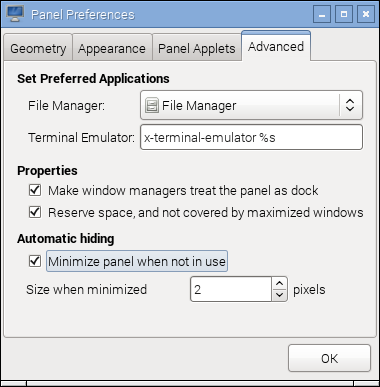
\includegraphics[scale=.35]{hide-task-bar.png} 
					\end{center}
					\caption{Chọn Minimize panel when not in use}\label{Fig:hide-task-bar}
				\end{figure}
			\end{itemize}
	\end{itemize}
\end{document}